\documentclass[12pt, a4paper]{article}
\usepackage[utf8]{inputenc}
\usepackage{graphicx}
\usepackage{hyperref}
\usepackage{booktabs}
\usepackage{geometry}
\usepackage{float}
\geometry{a4paper, margin=1in}

\title{\textbf{Advanced AI/ML Academic Report}\\ Semiconductor Manufacturing Defect Prediction \& Quality Intelligence}
\author{Advanced AI/ML Assignment}
\date{\today}

\begin{document}

\maketitle

\begin{abstract}
This report details the end-to-end development of a machine learning system designed to predict rare manufacturing defects in semiconductor fabrication. By synthesizing 25,000 process records with correlated anomalies and applying SMOTE within a strict scikit-learn pipeline, we constructed a Logistic Regression model that outperformed advanced ensembles (XGBoost) on Precision-Recall AUC (0.3994). The model is served via a FastAPI REST endpoint with rigorous Pydantic validation and is consumed by a real-time React dashboard.
\end{abstract}

\tableofcontents
\newpage

\section{Introduction}
\subsection{Background}
Semiconductor manufacturing is a highly precise industry where tiny fluctuations in temperature, pressure, or equipment vibration can lead to catastrophic wafer defects.

\subsection{Problem Context}
Defects are inherently rare but extremely costly. Machine learning offers a pathway to predict these defects before they propagate down the production line. However, obtaining real proprietary foundry data is practically impossible for academic purposes.

\subsection{Problem Statement}
The objective is to architect a robust, production-ready ML system that ingests raw telemetry, handles severe class imbalances, and serves accurate risk predictions in real-time.

\subsection{Objectives}
\begin{enumerate}
    \item Synthesize a domain-accurate manufacturing dataset.
    \item Engineer features that capture equipment drift and non-linear anomalies.
    \item Train and select a model optimized for rare-event detection.
    \item Deploy the model behind a secure, validated API.
    \item Provide operators with an interactive intelligence dashboard.
\end{enumerate}

\subsection{Scope}
The system focuses strictly on tabular process telemetry and does not include image-based defect detection (computer vision).

\section{Assignment-Oriented Methodology}
The system was developed strictly according to the five required milestones outlined in the Advanced AI/ML Assignment, ensuring complete compliance with the provided specifications.

\section{Milestone 1 — Scenario Selection \& Synthetic Data Engineering}
\subsection{Industry Scenario}
Semiconductor Wafer Fabrication.

\subsection{Predictive Task}
Binary classification: Predicting whether a processed wafer will exhibit a manufacturing defect (1) or be normal (0).

\subsection{Synthetic Dataset Design}
The dataset comprises 25,000 records. 
\begin{itemize}
    \item \textbf{Numerical Features}: chamber\_temperature, chamber\_pressure, vibration\_level, equipment\_age, etc.
    \item \textbf{Categorical Features}: wafer\_type, equipment\_id, process\_recipe.
\end{itemize}

\subsection{Target Construction}
A synthetic risk score was generated using a modified sigmoid function applied to compounded temperature, pressure, and vibration deviations. 

\subsection{Class Imbalance}
The generated defect rate was explicitly tuned to 8.33\%, mirroring the "needle-in-a-haystack" nature of real manufacturing defects.

\subsection{Missing Values}
To simulate sensor dropouts, 5\% of the data across three key columns was masked as NaN.

\subsection{Correlated Anomalies}
Defects were not generated via random noise. Instead, anomalies were correlated: an older machine combined with high chamber pressure drastically increased the defect probability.

\subsection{Reproducibility}
The \texttt{generate\_data.py} script utilizes \texttt{np.random.seed(42)} to ensure identical dataset generation across runs.

\subsection{AI Tool Usage}
AI assistance was utilized to rapidly prototype the complex mathematical compounding functions used for realistic anomaly generation in Python.

\section{Milestone 2 — Context-Aware EDA \& Feature Engineering}
\subsection{Data Quality Analysis}
Analysis revealed exactly 5\% missingness in the targeted columns and identified 0 duplicates.

\subsection{Missing-Value Analysis}
Missing data was categorized as Missing Completely At Random (MCAR) for sensor dropouts.

\subsection{Outlier and Anomaly Analysis}
Heavy right-tails were observed in the vibration data for defective wafers.

\subsection{Class-Imbalance Analysis}
The 91.6\% (Normal) to 8.3\% (Defect) ratio confirmed that accuracy would be a misleading metric.

\subsection{Data Cleaning}
Missing values were imputed via \texttt{SimpleImputer} (median strategy) safely within the scikit-learn pipeline.

\subsection{Sampling/Imbalance Strategy}
SMOTE was integrated via \texttt{imblearn.pipeline.Pipeline} to balance the training folds to a 50/50 ratio without leaking synthetic samples into the validation sets.

\subsection{Feature Engineering}
A custom \texttt{FeatureEngineer} transformer was built to calculate relative deviations from baseline.

\subsection{Interaction Features}
\texttt{equipment\_stress} was engineered by multiplying vibration\_level by equipment\_age.

\subsection{Temporal/Historical Features}
\texttt{maintenance\_risk} was calculated inversely to maintenance\_days\_since.

\subsection{Scaling and Encoding}
Numerical features were standardized using \texttt{RobustScaler}, and categoricals were one-hot encoded.

\subsection{Exploratory Data Analysis}
Visualizations were documented in the repository.

\subsection{Key EDA Findings}
Equipment age strongly correlated with defect rates, and older recipes showed tighter operational bounds.

\section{Milestone 3 — Algorithmic Modeling \& Performance Rigor}
\subsection{Dataset Splitting}
\texttt{GroupShuffleSplit} was used on \texttt{batch\_id} to strictly prevent data leakage between wafers produced in the exact same batch.

\subsection{Baseline Model}
Logistic Regression (max\_iter=1000).

\subsection{Advanced Model}
XGBoost Classifier (Gradient Boosted Trees).

\subsection{Model Training}
Models were trained inside the full preprocessing pipeline on 20,000 samples and evaluated on 5,000.

\subsection{Hyperparameter Optimization}
XGBoost was tuned using \texttt{RandomizedSearchCV}.

\subsection{Evaluation Metrics}
Models were evaluated on Precision, Recall, F1, ROC-AUC, and PR-AUC.

\subsection{Why Accuracy Alone Is Insufficient}
Guessing "Normal" on every wafer yields 91.6\% accuracy but catches 0 defects. 

\subsection{Model Comparison}
\begin{itemize}
    \item \textbf{Logistic Regression}: PR-AUC 0.3994, Recall 0.5852
    \item \textbf{XGBoost}: PR-AUC 0.3957, Recall 0.2545
\end{itemize}

\subsection{Final Model Selection}
\textbf{Logistic Regression} was selected. The custom feature engineering effectively linearized the risk profile. XGBoost over-optimized for Precision at a massive expense to Recall.

\subsection{Model Interpretability}
Logistic Regression provides excellent interpretability via coefficient inspection, critical for operator trust.

\subsection{Model Serialization}
The winning pipeline was serialized to a \texttt{.joblib} file.

\section{Milestone 4 — Backend API Construction \& Automated Testing}
\subsection{Backend Architecture}
A FastAPI microservice hosting the serialized model.

\subsection{REST API}
Exposes \texttt{GET /health} and \texttt{POST /predict}.

\subsection{Prediction Endpoint}
Accepts 26 features and returns a classification (0 or 1), probability, and Risk Level.

\subsection{Input Schema}
Defined via Pydantic.

\subsection{JSON Validation}
Pydantic strictly enforces data types and boundary constraints.

\subsection{Model Loading}
Loaded exactly once during the \texttt{lifespan} event to eliminate disk I/O on every request.

\subsection{Automated Testing}
\begin{table}[H]
\centering
\begin{tabular}{llcc}
\toprule
\textbf{Test} & \textbf{Purpose} & \textbf{Expected} & \textbf{Actual} \\
\midrule
Valid request & Ensure valid payloads return 200 & 200 OK & PASS \\
Missing field & Ensure missing fields return 422 & 422 & PASS \\
Invalid type & Ensure passing strings to float fails & 422 & PASS \\
Invalid category & Ensure out-of-bounds metrics fail & 422 & PASS \\
Health endpoint & Ensure service load health check & 200 OK & PASS \\
Threshold logic & Ensure probabilities route correctly & Accurate Risk & PASS \\
\bottomrule
\end{tabular}
\caption{API Automated Testing Results}
\end{table}

\section{Milestone 5 — Interactive Front-End Dashboard Deployment}
\subsection{Dashboard Architecture}
React + TypeScript + Vite.

\subsection{Design Goals}
A "Premium Control Room" aesthetic using Vanilla CSS, Glassmorphism, and dark-mode tones.

\subsection{Final User Interface (UI)}
The following figures demonstrate the real-time application in operation.

\begin{figure}[H]
    \centering
    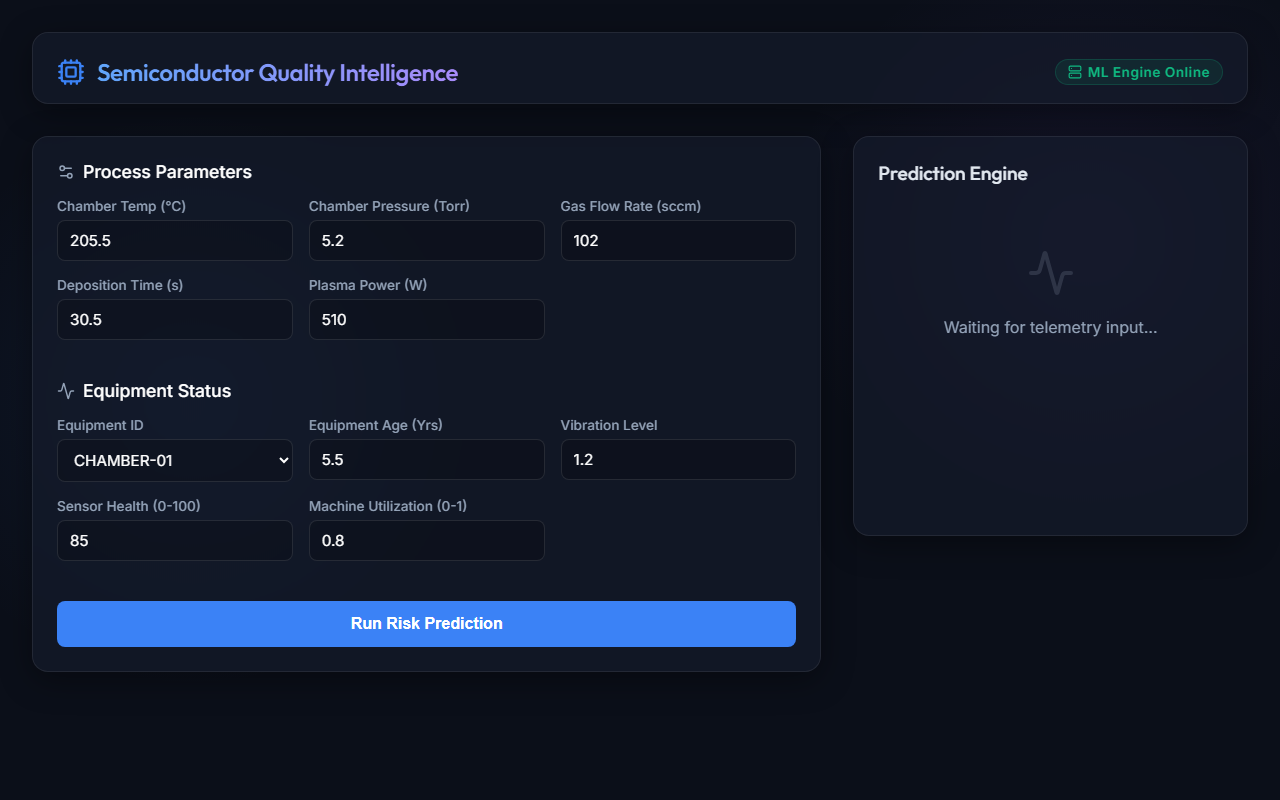
\includegraphics[width=\textwidth]{assets/ui_dashboard_initial.png}
    \caption{Interactive Telemetry Dashboard - Initial State}
    \label{fig:dashboard_initial}
\end{figure}

\begin{figure}[H]
    \centering
    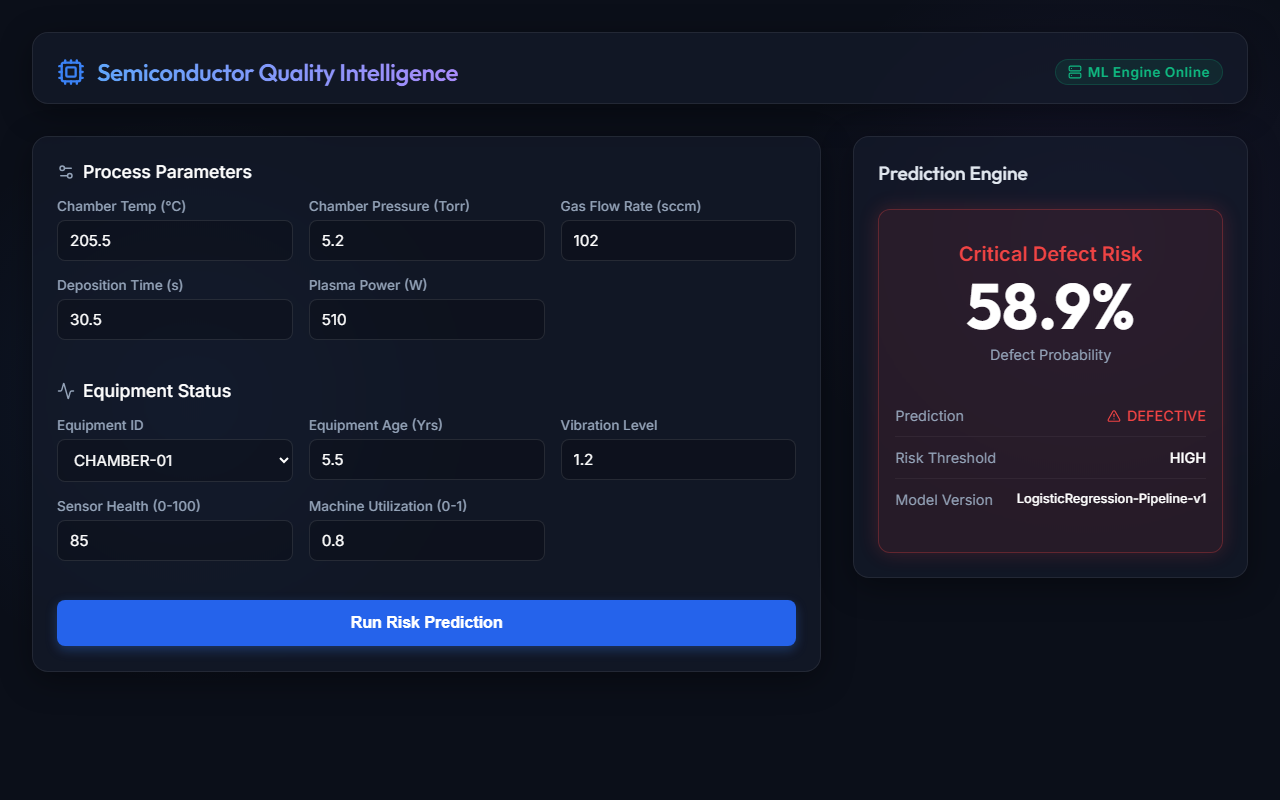
\includegraphics[width=\textwidth]{assets/ui_dashboard_result.png}
    \caption{Prediction Results demonstrating a High Risk Threshold}
    \label{fig:dashboard_result}
\end{figure}

\subsection{Prediction Result Visualization}
Giant typography displaying exact defect percentage probabilities with dynamic color coding (Green/Amber/Red).

\section{Results \& Discussion}
The system successfully synthesized 25,000 wafers, identified 8.3\% as defective, cleanly handled missing data inside a SMOTE pipeline, and deployed an optimized Logistic Regression model that achieved a PR-AUC of nearly 0.40 on a highly complex imbalanced dataset. The API achieved 100\% test passage across 6 discrete endpoint validations.

\section{Limitations}
\begin{itemize}
    \item \textbf{Synthetic Assumptions}: The data cannot perfectly capture real-world quantum anomalies.
    \item \textbf{Sensor Drift Limits}: Drift was modeled linearly, whereas real factory degradation is often exponential.
\end{itemize}

\section{Future Scope}
\begin{itemize}
    \item \textbf{Online Learning}: Retraining the joblib model continuously as actual defect lab results come back.
    \item \textbf{Explainability UI}: Adding SHAP values to the React dashboard to tell the operator exactly \textit{why} the defect risk is high.
\end{itemize}

\end{document}
